\subsection{Caso d'uso UC6: Stampa presentazione}
\begin{figure}[h] 
	\centering 
	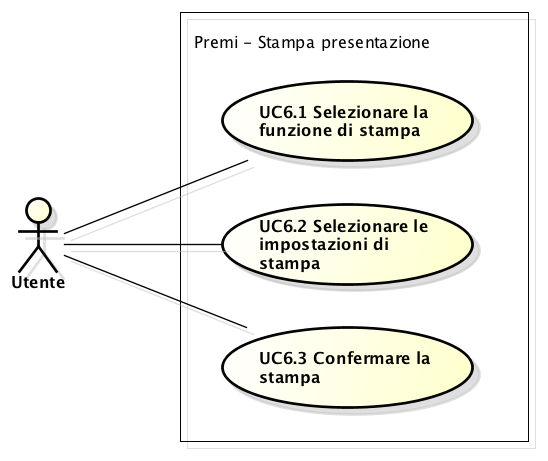
\includegraphics[scale=0.45] {img/UC6.png} 
	\caption{UC6 - Stampa presentazione} 
\end{figure}

\begin{itemize}
	\item \textbf{Attori:} Utente;
	\item \textbf{Scopo e descrizione:} L'utente ha creato una presentazione slide e vuole stamparla;
	\item \textbf{Precondizione:} Il sistema è in attesa che l'utente selezioni la funzione stampa;
	\item \textbf{Flusso degli eventi:}
	\begin{enumerate}
		\item L'utente seleziona la funzione stampa [UC6.1];
		\item L'utente seleziona le impostazioni di stampa [UC6.2];
		\item L'utente conferma la stampa [UC6.3].
	\end{enumerate}
	\item \textbf{Postcondizione:} Il sistema ha mandato in stampa la presentazione.
\end{itemize}

\subsection{Caso d'uso UC6.1: Selezionare la funzione di stampa}
\begin{itemize}
	\item \textbf{Attori:} Utente;
	\item \textbf{Scopo e descrizione:} L'utente seleziona dall'apposito menù la funzione di stampa per stampare la presentazione;
	\item \textbf{Precondizione:} Il sistema è in attesa che l'utente selezioni la funzione stampa;
	\item \textbf{Postcondizione:} Il sistema apre la finestra di dialogo per la stampa.
\end{itemize}

\subsection{Caso d'uso UC6.2: Selezionare le impostazioni di stampa}
\begin{figure}[h] 
	\centering 
	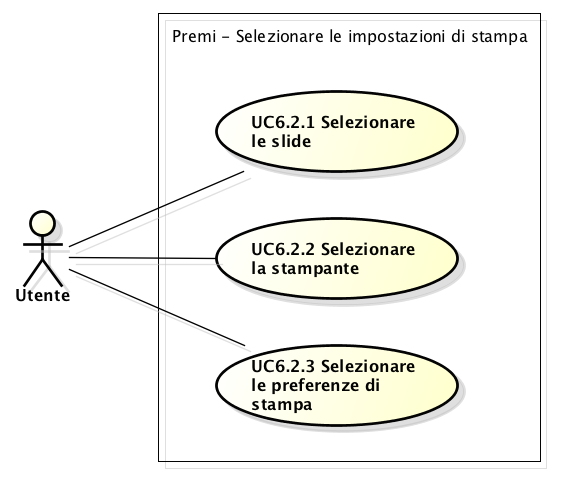
\includegraphics[scale=0.45] {img/UC6.2.png} 
	\caption{UC6.2 - Selezione impostazioni di stampa} 
\end{figure}

\begin{itemize}
	\item \textbf{Attori:} Utente;
	\item \textbf{Scopo e descrizione:} L'utente deve selezionare le impostazioni per la stampa della presentazione;
	\item \textbf{Precondizione:} Il sistema permette all'utente di selezionare le impostazioni desiderate;
	\item \textbf{Flusso di eventi:}
	\begin{enumerate}
		\item L'utente seleziona quali slide stampare [UC6.2.1]
		\item L'utente seleziona quale stampante usare [UC6.2.2]
		\item L'utente seleziona le preferenze di stampa fornite dalla stampante[UC6.2.3]
	\end{enumerate}
	\item \textbf{Postcondizione:} Il sistema registra tutte le impostazioni selezionate dall'utente.
\end{itemize}

	\subsection{Caso d'uso UC6.2.1: Selezionare le slide}
	\begin{itemize}
		\item \textbf{Attori:} Utente;
		\item \textbf{Scopo e descrizione:} L'utente seleziona se stampare tutte le slide della presentazione oppure solo una parte;
		\item \textbf{Precondizione:} Il sistema è in attesa che l'utente selezioni quali slide stampare;
		\item \textbf{Postcondizione:} Il sistema registra la scelta fatta dall'utente.
	\end{itemize}
	
	\subsection{Caso d'uso UC6.2.2: Selezionare la stampante}
	\begin{itemize}
		\item \textbf{Attori:} Utente;
		\item \textbf{Scopo e descrizione:} L'utente seleziona quale stampante installata nel sistema usare;
		\item \textbf{Precondizione:} Il sistema è in attesa che l'utente selezioni la stampante da usare;
		\item \textbf{Postcondizione:} Il sistema registra la scelta fatta dall'utente.
	\end{itemize}
	
	\subsection{Caso d'uso UC6.2.3: Selezionare le preferenze di stampa}
	\begin{itemize}
		\item \textbf{Attori:} Utente;
		\item \textbf{Scopo e descrizione:} L'utente seleziona le preferenze di stampa fornite dai driver della stampante stessa;
		\item \textbf{Precondizione:} Il sistema è in attesa che l'utente selezioni le preferenze da usare;
		\item \textbf{Postcondizione:} Il sistema registra la scelte fatte dall'utente.
	\end{itemize}


\subsection{Caso d'uso UC6.3: Confermare la stampa}
\begin{itemize}
	\item \textbf{Attori:} Utente;
	\item \textbf{Scopo e descrizione:} L'utente conferma la stampa della presentazione;
	\item \textbf{Precondizione:} Il sistema ha ricevuto la richiesta di stampa della presentazione;
	\item \textbf{Postcondizione:} Il sistema ha mandato in stampa la presentazione.
\end{itemize}

\newpage